%
% Example based on documentation for the songs project:
% http://songs.sourceforge.net/
%
\documentclass[10pt, openany]{book}

\usepackage[utf8]{inputenc}
\usepackage[spanish]{babel}
\usepackage[chorded]{songs}


%\usepackage[letterpaper, margin=2.5cm]{geometry} % Reduce los márgenes
\noversenumbers

\newindex{titleidx}{cbtitle}
\newauthorindex{authidx}{cbauth}
\newscripindex{scripidx}{cbscrip}
\newindex{zambasidx}{zambas}
\newindex{chacarerasidx}{chacareras}

\usepackage{titlesec}
\usepackage{hyperref} 


%\titleformat{\chapter}[display]
%{\normalfont\bfseries}{}{0pt}{\Huge}
\newcommand{\authorname}{Cantus Vetus}
\newcommand{\translatorname}{Francisco Sesto}
\newcommand{\booktitle}{El libro del Folklore}
\newcommand{\subtitle}{Bien Argentino}
\newcommand{\publisher}{Argentina}
\newcommand{\editionyear}{2024}
\newcommand{\isbn}{}
\title{\booktitle}
\author{\authorname}
\usepackage{misc/options}

%\renewcommand{\stitlefont}{
%	\Roman\Large\baselineskip=20pt\lineskiplimit=0pt
%}

\renewcommand{\stitlefont}{
	\Roman\Large\baselineskip=20pt\lineskiplimit=0pt
}
%\renewcommand{\printchord}[1]{{\color{red!70!black}#1}}
\newcommand\lmr{\fontfamily{lmr}\selectfont}    


\noversenumbers

\renewcommand\printchord[1]{{\lmr\small\sffamily\color{red!70!black}#1}}

\begin{document}
	% Mostrar el índice de títulos de canciones
%	\showindex{Índice de Canciones}{titleidx}
	% Mostrar el índice de autores
	% Mostrar el índice de referencias a escritura
%	\showindex{Índice de Referencias a Escritura}{scripidx}
    \frontmatter
    \pagestyle{empty}

% Capa
\begin{center}
\begin{tikzpicture}[remember picture,overlay]

    % Proporção áurea
    %\pgfmathsetmacro{\goldenheight}{\paperwidth / \goldenratio}
    %\pgfmathsetmacro{\goldenwidth}{\paperwidth}

    % Fundo preto
    \fill[black] (current page.south west) rectangle (current page.north east);

    % Autor
    \node[white, font=\Huge, anchor=north, text width =\linewidth, align = center] (author) at ([yshift=-44pt] current page.north) {\textcolor{customgold}{\scshape\large\authorname}};

    % Título
    \node[white, font=\Large, anchor=north, text width =0.9\linewidth, align = center, below=4pt of author.south] (title) {\scshape\Huge\booktitle};

    % Subtítulo
    \ifx\subtitle\undefined\else\if\relax\detokenize\expandafter{\subtitle}\relax\else
    {\node[white, font=\Large, text width =\linewidth, align = center, anchor=north, below=8pt of title.south] {\textcolor{lightgray}{\scshape\large\subtitle}};}
    \fi\fi

    % Padrão de círculos central
    \begin{scope}[shift={(current page.center)}, scale=1.0871]
        \foreach \x in {-20, -18, -16, -14, -12, -10, -8, -6, -4, -2, 0, 2, 4, 6, 8, 10, 12, 14, 16, 18} {
            \foreach \y in {-2, 2} {
                \begin{scope}[shift={(\x + 1, \y)}]
                    \foreach \r in {0.2, 0.4, 0.6, 0.8, 1.0} {
                        \draw[thick, darkgray] (0,0) circle (\r);
                    }
                \end{scope}
            }
            \foreach \y in {-3, -1, 1, 3} {
                \begin{scope}[shift={(\x, \y)}]
                    \foreach \r in {0.2, 0.4} {
                        \draw[thick, darkgray] (0,0) circle (\r);
                    }
                \end{scope}
            }
            \foreach \y in {-1, 1} {
                \begin{scope}[shift={(\x, 0)}]
                    \foreach \r in {0.2, 0.4, 0.6, 0.8, 1.0} {
                        \draw[thick, customgold] (0,0) circle (\r);
                        \fill[thick, customgold] (0,0) circle (\r);
                    }
                \end{scope}
            }
            \foreach \y in {-1, 1} {
                \begin{scope}[shift={(\x, \y)}]
                    \foreach \r in {0.2, 0.4, 0.6, 0.8, 1.0} {
                        \fill[black] (0,0) circle (\r);
                    }
                \end{scope}
            }
            \foreach \y in {-1, 1} {
                \begin{scope}[shift={(\x, \y)}]
                    \foreach \r in {0.2, 0.4, 0.6, 0.8, 1.0} {
                        \draw[thick, darkgray] (0,0) circle (\r);
                    }
                \end{scope}
            }
        }
    \end{scope}

    % Editora
    \node[white, font=\Huge, anchor=south] (publisher) at ([yshift=32pt] current page.south) {\textcolor{gray}{\scshape\large\publisher}};

    % Logotipo da editora
    \node[anchor=north, above=4pt of publisher.north] {
\includegraphics[width=0.07\textwidth]{frontmatter/logo-white.png}};

    % Outras informações
    \ifx\translatorname\undefined
    \else
        \if\relax\detokenize\expandafter{\translatorname}\relax
        \else{   
            \node[white, font=\Large, anchor=north, above=114pt of publisher.north] (translatedBy) {\textcolor{gray}{\itshape\large{Recopilado por}}};
            
            \node[white, font=\Large, anchor=south, below=2pt of translatedBy.south] (translatorAuthor) {\textcolor{lightgray}{\itshape\large\translatorname}};       
            }
        \fi
    \fi        
\end{tikzpicture}
\end{center}

\cleardoublepage

% Página de título (contra-capa)
\begin{titlepage}
	\centering
	\newgeometry{top=1in,bottom=1in,right=0in,left=0in}
    \thispagestyle{empty}
	~	
    % Autor
	\vspace{24pt}
	{\scshape\large \authorname\par}

    % Título
	\vspace{6pt}
	{\scshape\Huge \booktitle\par}

    % Subtítulo
    \ifx\subtitle\undefined\else\if\relax\detokenize\expandafter{\subtitle}\relax\else
    {\vspace{6pt}
	{\scshape\large \subtitle\par}
 
	\vspace{\stretch{1.25}}}
    \fi\fi
    
    % Quem fez a tradução
    \ifx\translatorname\undefined\else\if\relax\detokenize\expandafter{\translatorname}\relax\else
    {{\itshape\large{Recopilado por}\par}
	\vspace{6pt}

    {\itshape\Large\translatorname\par}}
    \fi\fi

    % Editora
    \vspace{\stretch{6}}
	{\Huge\scshape\large\publisher\par}
\end{titlepage}
      % Página de título
    % Página de copyright

{\small
\setlength{\parindent}{0em}\setlength{\parskip}{1em}
~
\vfill

% Data da primeira publicação
Primera edición, \editionyear{}

% Copyright
Copyright \copyright{} 2024 \authorname

% Texto resumido da licença
El folklore argentino es una rica expresión de nuestra historia y tradiciones. Con este proyecto, nos proponemos rescatar y poner en valor las canciones que han marcado a varias generaciones, contribuyendo así a mantener viva nuestra cultura popular y a fomentar el aprecio por nuestras raíces. Este proyecto es una construcción colectiva. Si tienes alguna sugerencia o corrección, por favor, comparte tus conocimientos escribiéndome a sestofrancisco@gmail.com.

% ISBN, se houver
\ifx\isbn\undefined\else\if\relax\detokenize\expandafter{\isbn}\relax\else{ISBN \isbn{}}\fi\fi

% Logotipo da editora
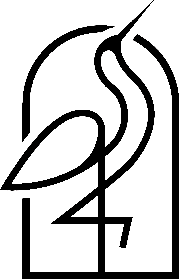
\includegraphics[width=0.07\linewidth]{frontmatter/logo-black.png}

% Editora
Publicado por \publisher{}
}
  % Página de direitos autorais
    % Prefácio
\chapter{Prefacio}

\lettrine{E}{l folklore argentino}, rico y diverso como el territorio que lo vio nacer, es el resultado de un largo proceso histórico y cultural que se remonta a los albores de nuestra nación. Para entender cómo llegó el folklore a Argentina, debemos viajar en el tiempo y explorar las múltiples corrientes que confluyeron en nuestras tierras.

Los orígenes del folklore argentino se pueden trazar hasta las culturas indígenas que habitaban estas tierras mucho antes de la llegada de los europeos. Estos pueblos originarios, con sus ritmos, instrumentos y tradiciones orales, sentaron las primeras bases de lo que luego se convertiría en nuestro folklore.
Con la llegada de los conquistadores españoles en el siglo XVI, se produjo un encuentro cultural que transformaría para siempre el panorama musical y cultural de la región. Los europeos trajeron consigo instrumentos como la guitarra, que se convertiría en un elemento icónico de nuestro folklore, así como formas musicales y poéticas que se fusionarían con las tradiciones locales.

No podemos olvidar la influencia africana, que llegó con los esclavos traídos durante la época colonial. Sus ritmos y tradiciones se entrelazaron con las ya existentes, enriqueciendo aún más el tapiz cultural en formación.

A lo largo de los siglos XVIII y XIX, mientras Argentina se forjaba como nación, el folklore continuó evolucionando. Las vastas llanuras de la pampa vieron nacer la figura del gaucho, cuyas payadas y milongas se convertirían en pilares de nuestra tradición folklórica. En el noroeste, la influencia andina dio lugar a ritmos como la zamba y la chacarera, mientras que en el litoral, la chamamé reflejaba la fusión de elementos guaraníes y europeos.

La inmigración masiva de finales del siglo XIX y principios del XX trajo consigo nuevas influencias, principalmente de Italia y Europa del Este, que se integraron al ya rico panorama cultural argentino. Este crisol de culturas contribuyó a la diversidad y riqueza de nuestro folklore.

Es importante destacar que el folklore argentino no es un fenómeno estático, sino un organismo vivo que ha seguido evolucionando hasta nuestros días. A lo largo del siglo XX, figuras como Atahualpa Yupanqui, Mercedes Sosa y otros grandes artistas llevaron nuestra música folklórica a los escenarios del mundo, consolidando su lugar en el panorama cultural global.

En este libro, exploraremos cómo todas estas influencias se han entretejido para crear el rico tapiz del folklore argentino que conocemos hoy. Desde las danzas tradicionales hasta las canciones que han marcado generaciones, desde los instrumentos autóctonos hasta las leyendas que se transmiten de boca en boca, cada elemento nos cuenta una parte de nuestra historia colectiva.
\cleardoublepage   % Make sure contents page starts on right-side page        % Prefácio
    \tableofcontents 
    
%    \tableofcontents\thispagestyle{empty}\cleardoublepage        % Sumário
    
    % Main matter
    \mainmatter
    \pagestyle{fancy}  

	\chapter{Zambas}
	 \newpage
	
	\begin{songs}{zambasidx}
		
	
 
\beginsong{Agitando Pañuelos}[by={Adolfo Ábalos}]

		\phantomsection  \addcontentsline{toc}{section}{Agitando Pañuelos} 
 \label{sec:Agitando_Pañuelos} \beginverse
		\[Em]Te \[E7]vi, no olvida\[Am]ré un carna\[D7]val, guitarra, bombo y vio\[G]lín \[B7] \\
		\[Em]Agitando pa\[D]ñuelos te \[C]vi, cadencia al \[B7]bailar, airosa el \[Am]perfil \[G] \[B7] \[Em] \\
		\endverse
		
		\beginverse
		\[E7]Me \[Am]fui diciendo a\[D7]diós y en ese a\[G]diós quedó enredado un \[B7]querer \\
		\[Em]Agitando pa\[D]ñuelos me \[C]fui ¡Qué lindo \[B7]añorar tu zamba de \[Am]ayer! \[G] \[B7] \[Em] \\
		\endverse
		
		\beginchorus
		\[Em]Yo me \[E7]iré tu ven\[Am]drá Yo te lle\[D7]varé, mi rancho se alegre\[G]rá \[B7] \\
		\[Em]Agitando pa\[D]ñuelos me \[C]iré y en mí vivi\[B7]rá aquel carna\[Am]val \[G] \[B7] \[Em] \\
		\[Em]Agitando pa\[D]ñuelos me \[C]iré cantando esta \[B7]zamba repiquetea\[Am]dita \[G] \[B7] \[Em]
		\endchorus
		
		\beginverse
		\[Em]Vol\[E7]ví y te encon\[Am]tré... toda mi \[D7]voz le dio a la copla un can\[G]tar \[B7] \\
		\[Em]Agitando pa\[D]ñuelos vol\[C]ví, sintiendo \[B7]también mi pecho agi\[Am]tar \[G] \[B7] \[Em] \\
		\endverse
		
		\beginverse
		\[E7]Bai\[Am]lé hasta el fi\[D7]nal... engualicha\[G]o, bailé hasta el amane\[B7]cer \\
		\[Em]Agitando pa\[D]ñuelos bai\[C]lé. ¡Qué lindo \[B7]bailar las zambas de \[Am]ayer! \[G] \[B7] \[Em] \\
		\endverse
		
		\endsong
		
 
\beginsong{Al Jardín De La República}[by={Virgilio Carmona}]

		\phantomsection  \addcontentsline{toc}{section}{Al Jardín De La República} 
 \label{sec:Al_Jardín_De_La_República} \beginverse
		\[G]Desde el \[D7]norte traigo en el \[G]alma \\
		\[D7]la alegre \[G]zamba que canto a\[D7]quí \\
		\[G]y que \[B7]bailan los tucu\[Em]manos \\
		\[B7]con entusiasmo \[Em]propio de \[D]allí, \\
		\[C]cada \[B7]cual sigue a su pa\[Em]reja, \\
		\[B7]joven o vieja, \[Em]de todo vi.
		\endverse
		
		\beginverse
		\[G]Media \[D7]vuelta y la compa\[G]ñera \\
		\[D7]forma una \[G]rueda para se\[D7]guir, \\
		\[G]viene el \[B7]gaucho, le hace un flo\[Em]reo \\
		\[B7]y un zapateo co\[Em]mienza \[D]allí, \\
		\[C]sigue el \[B7]gaucho con su flo\[Em]reo \\
		\[B7]y el zapateo ter\[Em]mina allí.
		\endverse
		
		\beginchorus
		\[Em]Para las \[E7]otras \[Am]no, \\
		\[C]Pa' las del \[B7]norte \[Am]sí, \\
		\[B7]para las Tu\[Em]cumanas, \\
		\[B7]mujer ga\[Em]lana, \[D]naranjo en \[C]flor \\
		\[B7]todo lo que ellas \[Em]quieran \\
		\[B7]que la primera ya \[Em]terminó.
		\endchorus
		
		\beginverse
		\[G]No me \[D7]olvido, viera, com\[G]padre, \\
		\[D7]de aquellos \[G]bailes que hacen a\[D7]llí \\
		\[G]tucuma\[B7]nos y tucuma\[Em]nas, \\
		\[B7]todos se afanan por \[Em]diver\[D]tir \\
		\[C]y hacer \[B7]linda esta triste \[Em]vida, \\
		\[B7]así se olvida que \[Em]hay que morir.
		\endverse
		
		\beginverse
		\[G]Empa\[D7]nadas y vino en \[G]jarra, \\
		\[D7]una gui\[G]tarra, bombo y vio\[D7]lín, \\
		\[G]y unas \[B7]cuantas mozas bi\[Em]zarras \\
		\[B7]pa' que la farra pueda \[Em]se\[D]guir \\
		\[C]sin que \[B7]falten esos cole\[Em]ros, \\
		\[B7]viejos cuenteros, \[Em]pa' que hagan reír.
		\endverse
		\endsong
 
\beginsong{De Mi Madre}[by={José Ignacio Rodríguez}]
    \phantomsection  \addcontentsline{toc}{section}{De Mi Madre} 
 \label{sec:De_Mi_Madre} \beginverse
    \[C]Volveré... \[G7]Volveré...
    Me espera la \[C]noche, vestida de \[G7]azul \\
    Y hasta el arro\[E7]yito que baja del \[Am]cerro,
    tra\[F]erá recu\[C]erdos de m\[G7]i ju\[C]ventud  \\
    \endverse

    \beginverse
    \[C]Volveré... \[G7]Volveré...
    Donde está mi \[C]madre esperándome\[G7]... \\
    De nuevo en sus [E7]brazos volver a ser \[Am]niño,
    viv\[F]ir como \[C]solo se v\[G7]ive una \[C]vez \\
    \endverse

    \beginchorus
    \[F]Azahar de blancos \[C]jazmines,
              \[G7]que aroman el patio del \[C]viejo jardín \\
           \[E7]Un beso de luna, me \[Am]espera en los valles,
    mi \[F]rancho, mi \[C]madre, todo mi \[G7]sentir \[C] \\
    \endchorus

    \beginverse
    \[C]Volveré... \[G7]Volveré...
    Por ese ca\[C]mino que ayer me ale\[G7]jó \\
    Al rumbo del \[E7]ave que vuelve a su \[Am]nido,
    busca\[F]ndo un \[C]alivio pa\[G7]ra su \[C]dolor  \\
    \endverse

    \beginverse
    \[C]Volveré... \[G7]Volveré...
    Y lejos la \[C]noche repite mi \[G7]voz \\
    La voz de un \[E7]cariño que lejos se \[Am]siente,
    y ll\[F]ama al \[C]ausente de su co\[G7]razón \[C] \\
    \endverse

\endsong
 
\beginsong{La Pomeña}[by={Cuchi Leguizamón}]
		\transpose{-3}

		\phantomsection  \addcontentsline{toc}{section}{La Pomeña} 
 \label{sec:La_Pomeña} \beginverse
		\[G7M]Eulogia Tapia en \[Em]La Poma \[Am6]
		Al \[Am7]aire \[D7]da su ter\[G7M]nura \\
		\[Dm7]Si pasa sobre la \[Db7]arena \[C7M/G]
		Iba pi\[Am6]sando la \[D7]luna \[G7M] \\
		\[F7]Si pasa sobre la \[E7]arena \[A6]
		Iba pi\[Am6]sando la luna \[G#7M] \[G7M]
		\endverse
		
		\beginverse
		\[G7M]El trigo que va cor\[Em]tando \[Am6]
		Ma\[Am7]dura \[D7]por su cin\[G7M]tura \\
		\[Dm7]Mirando flores de \[Db7]alfalfa \[C7M/G]
		Sus ojos \[Am6]negros se a\[D7]zulan \[G7M] \\
		\endverse
		
		\beginchorus
		\[G]El sauc\[G/F#]e de tu ca\[F7]sa 
		Te está llo\[E]rando \[Am6] \\
		\[Cm7]Por qué te roban Eu\[F7]logia \[Bm7]
		Carnava\[D7sus4]leando \[G#7M] \[G7M] \\
		\[Bm]Por que te roban Eu\[E7(9)]logia \[Am6]
		Carnava\[D7]leando \[G#maj7] \[Gmaj7]
		\endchorus
		
		\beginverse
		\[G7M]La cara se le enha\[Em]rina \[Am6]
		La \[Am7]sombra \[D7]se le ena\[G7M]rena \\
		\[Dm7]Cantando y desenca\[Db7]ntando \[C7M/G]
		Se le entre\[Am6]veran las \[G#7M]penas \[G7M]
		\endverse
		
		\beginverse
		\[G7M]Viene en un caballo \[Em]blanco \[Am6]
		La \[Am7]caja \[D7]en sus manos \[G7M]tiembla \\
		\[Dm7]Y cuando se hunde en la \[Db7]noche \[C7M/G]
		Es una \[Am6]dalia mo\[G#7M]rena \[G7M]
		\endverse
		\endsong
 
\beginsong{La Tempranera}[by={Eduardo Falú}]
			
			\phantomsection  \addcontentsline{toc}{section}{La Tempranera} 
 \label{sec:La_Tempranera} \beginverse
			\[Em]Eras la temprane\[B7]ra \\
			niña pri\[E7]mera, amane\[Am]cida flor, \\
			suave rosa ga\[Em]lana \\
			la más bo\[F#7]nita Tucuma\[B7]na \[E7] \\
			\[Am]suave rosa ga\[Em]lana \\
			la más bo\[B7]nita Tucuma\[Em]na.
			\endverse
			
			\beginverse
			Frente de adoles\[B7]cente \\
			gentil mi\[E7]lagro de tu tri\[Am]gueña piel, \\
			negros ojos sin\[Em]ceros \\
			paloma \[F#7]tibia de Monte\[B7]ros \[E7] \\
			negros ojos sin\[Am]ceros \\
			paloma \[B7]tibia de Monte\[Em]ros.
			\endverse
			
			\beginchorus
			\[E7]Al bailar esta \[Am]zamba fue \\
			\[D7]que rendido te \[G]amé \[B7] \[E7] \\
			\[Am]Eras la temprane\[Em]ra \\
			de mis ar\[F#7]restos prisione\[B7]ra \[E7] \\
			\[Am]Mía... ya te sa\[Em]bía \\
			cuando por \[B7]fin te coro\[Em]né.
			\endchorus
			
			\beginverse
			Eras la prime\[B7]vera \\
			la pregone\[E7]ra del delic\[Am]ado amor, \\
			lloro amarga\[Em]mente \\
			aquel ro\[F#7]mance adolescen\[B7]te \[E7] \\
			lloro amarga\[Am]mente \\
			aquel ro\[B7]mance adolescen\[Em]te.
			\endverse
			\endsong
			
			
			
 
\beginsong{La Viajerita}[by={Atahualpa Yupanqui}]
			\phantomsection  \addcontentsline{toc}{section}{La Viajerita} 
 \label{sec:La_Viajerita} \beginverse
			\[Am]Desde los cerros \\
			\[Am]baja esta \[E7]zámbita, \\
			\[Am]por eso la llamo yo \\
			\[F]la viajerita, \[C]palomi\[E7]tay. \[Am]
			\endverse
			
			\beginverse
			\[Am]Sendas de \[E7]arena, \\
			\[Am]arcos flo\[E7]ridos, \\
			\[F]y un corazón que pena \\
			\[C]por un oli\[E7]vido, \[Am]palomi\[E7]tay. \[Am]
			\endverse
			
			\beginchorus
			\[G7]¡Ay, viajeri\[C]ta! \\
			\[G7]el alba a\[C]soma, \\
			\[F]trayendo de los cerros, \\
			\[C]frescor y a\[E7]roma, \[Am]palomi\[E7]tay. \[Am]
			\endchorus
			
			\beginverse
			\[Am]Yo soy de a\[E7]rriba, \\
			\[Am]soy de Go\[E7]chula, \\
			\[F]ranchitos, montes, ríos, \\
			\[C]soles y lu\[E7]nas, \[Am]palomi\[E7]tay. \[Am]
			\endverse
			
			\beginverse
			\[Am]Hasta el Pachi\[E7]vi, \\
			\[Am]voy los do\[E7]mingos, \\
			\[F]y por la noche al cerro, \\
			\[C]vuelvo soli\[E7]to, \[Am]palomi\[E7]tay. \[Am]
			\endverse
			\endsong
 
\beginsong{Luna Tucumana}[by={Atahualpa Yupanqui}]
		\phantomsection  \addcontentsline{toc}{section}{Luna Tucumana} 
 \label{sec:Luna_Tucumana} \beginverse
		\[E7]Yo no le canto a la \[Am]luna
		Porque \[E7]alumbra y nada \[Am]más \[A7] \\
		\[Dm]Le canto porque ella \[Am]sabe
		De mi largo \[E7]caminar \[Am] \\
		\endverse
		
		\beginverse
		\[E7]Hay lunita tucuma\[Am]na
		Tamborcito \[E7]calcha\[Am]quí \[A7] \\
		\[Dm]Compañera de los \[Am]gauchos
		En las sendas de \[E7]Tafí \[Am] \\
		\endverse
		
		\beginchorus
		\[G]Perdido en las cerra\[C]zones
		Quien sabe \[G7]vidita por \[F7]donde \[C]andaré \[A7] \\
		\[Dm]Mas cuando salga la \[Am]luna
		Canta\[E7]ré, canta\[Am]ré \[A7] \\
		\[Dm]A mi Tucumán que\[Am]rido
		Canta\[E7]ré, canta\[Am]ré, canta\[E7]ré \[Am]
		\endchorus
		
		\beginverse
		\[E7]Con esperanza o con \[Am]pena
		En los campos de \[E7]acheral \[Am] \[A7] \\
		\[Dm]Yo he visto a la luna \[Am]buena
		Besando el caña\[E7]veral \[Am] \\
		\endverse
		
		\beginverse
		\[E7]Si en algo nos parece\[Am]mos
		Luna de la so\[E7]ledad \[Am] \[A7] \\
		\[Dm]Yo voy andando y can\[Am]tando
		Que es mi modo de \[E7]alumbrar \[Am] \\
		\endverse
		
		\endsong
 
\beginsong{Saltita}[by={Roberto Ternán}]
		\phantomsection  \addcontentsline{toc}{section}{Saltita} 
 \label{sec:Saltita} \beginverse
		\[Am]Me sigue tu re\[F]cuerdo \[G7]por donde \[C]vaya \\
		\[D]Y en la zamba carpera m\[F]e llora el a\[G7]lm\[C]a \\
		\[E7]Y en la zamba car\[Am]pera, Saltita,  \[Dm]me ll\[C]ora \[E7]el al\[Am]ma.
		\endverse
		
		\beginverse
		Andando solo y \[F]lejos, \[G7]tierra de \[C]Güemes \\
		\[D]Lágrimas de nostalgias, br\[F]otan a\[G7]vec\[C]es \\
		\[E7]Lágrimas de nos\[Am]talgias, Saltita, b\[Dm]rot\[C]an a\[E7] ve\[Am]ces.
		\endverse
		
		\beginchorus
		\[F]Pura nostalgias teng\[C]o, \\
		\[D]cuando me acuerdo de \[C]Salta \\
		\[D]Por eso coca y vica nun\[F]ca me f\[G7]alt\[C]a \\
		\[E7]Soñando carnav\[Am]ales, Saltita, s\[Dm]e v\[C]uelve \[E7]mi al\[Am]ma.
		\endchorus
		
		\beginverse
		Desde la cruz del \[F]cerro \[G7]ya se adi\[C]vina \\
		\[D]que por tus calles corren, ca\[F]nto y p\[G7]oes\[C]ía \\
		\[E7]que por tus calles \[Am]corren, Saltita, c\[Dm]an\[C]to y p\[E7]oes\[Am]ía.
		\endverse
		
		\beginverse
		Digo tu nombre y \[F]suena \[G7]chura la \[C]zamba \\
		\[D]como para irse yendo d\[F]e cac\[G7]har\[C]pallas \\
		\[E7]como para irse \[Am]yendo, Saltita, d\[Dm]e c\[C]ach\[E7]arpal\[Am]las.
		\endverse
		\endsong
 
\beginsong{Zamba Del Laurel}[by={Cuchi Leguizamón}]
		\phantomsection  \addcontentsline{toc}{section}{Zamba Del Laurel} 
 \label{sec:Zamba_Del_Laurel} \beginverse
		\[G]Si lo verde tu\[E7]viera otro \[Am]nombre
		\[D7]Debería llamarse ro\[G]cío \\
		\[Bm7(b5)]Si pudiera vol\[E7]ver desde el \[Am]agua al laurel
		\[D7]Volvería a la in\[G]fancia del río
		\endverse
		
		\beginverse
		\[G]En lo verde lau\[E7]rel de tus \[Am]ojos
		\[D7]El misterio del bosque se a\[G]soma \\
		\[Bm7(b5)]Y la vida otra \[E7]vez vuelve \[Am]flor de tu piel
		\[D7]Bajo un sol de mu\[G]chacha y aroma
		\endverse
		
		\beginchorus
		\[C#m7(b5)]Déjame en lo \[F#7]verde celebrar el \[Bm7]día
		Porque por lo \[Am]verde regreso a la \[B7]vida \[Em] \\
		\[Cmaj7]Yo \[C#dim]muero para \[Bm7]volver
		Juntando ro\[Am]cío en la \[D7]flor del lau\[Dm]rel \[G7] \\
		\[Cmaj7]Yo \[C#dim]muero para \[G]volver
		Juntando ro\[Am]cío en la \[D7]flor del lau\[G]rel
		\endchorus
		
		\beginverse
		\[G]Si lo verde su\[E7]piera tu \[Am]nombre
		\[D7]La ternura no me olvida\[G]ría \\
		\[Bm7(b5)]Porque viene de \[E7]vos, puro y \[Am]simple el verdor
		\[D7]Como el simple ver\[G]dor de la vida
		\endverse
		
		\beginverse
		\[G]Se me ha vuelto co\[E7]gollo el si\[Am]lencio
		\[D7]De esperarte a la orilla del \[G]río \\
		\[Bm7(b5)]Y me gusta sa\[E7]ber que un a\[Am]roma a laurel
		\[D7]Te llenó de ro\[G]cío el olvido
		\endverse
		\endsong
 
\beginsong{Zamba Por Vos}[by={Alfredo Zitarrosa}]
    \phantomsection  \addcontentsline{toc}{section}{Zamba Por Vos} 
 \label{sec:Zamba_Por_Vos} \beginverse
             
    \[C]Yo no canto por vos \[G7]\\
    te canta la zamba \[C]\\
    y dice al cantar\[G7] \\
    no te pu\[F]edo olv\[C]idar \\
    no te pu\[G7]edo olvid\[C]ar.
    \endverse

    \beginverse
    \[C]Yo no canto por vos \[G7]\\
    te canta la zamba \[C]\\
    y cantando así\[G7] \\
    canta p\[F]ara m\[C]í \\
    canta pa\[G7]ra mí\[C].
    \endverse

    \beginchorus
    \[C7]Zambita canta\[F] \\
    no la esperes más \[C] \\
    tenés qu\[D]e pens\[G7]ar \\
    que si \[F]no volv\[C]ió \\
    es que y\[G7]a te olv\[C]idó \\
    perfum\[C]a esa fl\[G7]or \\
    que se ma\[F]rchi\[C]tó \\
    que se mar\[G7]chi\[C]tó.
    \endchorus

    \beginverse
    \[C]Yo tuve un amor \[G7]\\
    lo dejé esperando\[C] \\
    y cuando volv\[G7]í \\
    no l\[F]a conocí\[C] \\
    no l\[G7]a conocí.\[C]
    \endverse

    \beginverse
    \[C]Dijo que tal vez \[G7]\\
    me estuviera amando\[C] \\
    me miró y se fu\[G7]e \\
    sin d\[F]ecir por qué\[C] \\
    sin dec\[G7]ir por qu\[C]é.
    \endverse

 
\endsong
 
		
		
	\end{songs}
	
	\chapter{Chacareras}
	\newpage
	
	\begin{songs}{chacarerasidx}

%	\setcounter{songnum}{\thesongcount}	
	
 
\beginsong{Chacarera De Un Triste}[by={Hnos. Simón}]
		
		\phantomsection  \addcontentsline{toc}{section}{Chacarera De Un Triste} 
 \label{sec:Chacarera_De_Un_Triste} \beginverse
		\[Em]Para qué quiero vivir \\
		\[G]Con el corazón deshecho \\
		\[A]Para qué quiero la \[G]vida \\
		\[B7]después de lo que me has \[Em]hecho.
		\endverse
		
		\beginverse
		\[Em]Yo te di mi corazón \\
		\[G]vos el tuyo voz me entregaste \\
		\[A]con engaño y así el \[G]mío \\
		\[B7]prenda lo despedaz\[Em]aste.
		\endverse
		
		\beginverse
		\[Em]Ay por qué fuiste tan cruel \\
		\[G]si tu cariño esperaba \\
		\[A]por qué jugaste con \[G]migo \\
		\[B7]prenda si te idolatr\[Em]aba.
		\endverse
		
		\beginverse
		\[Em]Yo del mundo olvide \\
		\[G]desengaños y amarguras \\
		\[A]pero lo que vos me \[G]hiciste \\
		\[B7]prenda mi alma perd\[Em]ura.
		\endverse
		
		\beginverse
		\[Em]Seguí guitarra seguí \\
		\[G]seguí como yo llorando \\
		\[A]compañera hasta la \[G]muerte \\
		\[B7]seguí mi alma consola\[Em]ndo.
		\endverse
		
		\beginverse
		\[Em]No hay consuelo ya lo sé \\
		\[G]para que voy a buscarlo \\
		\[A]tan deshecha tengo el \[G]alma \\
		\[B7]que inútil será log\[Em]rarlo.
		\endverse
		
		\beginverse
		\[Em]Cantando me pasaré \\
		\[G]muy triste esta chacarera \\
		\[A]pueda ser que vos te \[G]acuerdes \\
		\[B7]en el momento que mu\[Em]era.
		\endverse
		
		\beginverse
		\[Em]Seguí guitarra seguí \\
		\[G]prenda por lo que me hiciste \\
		\[A]rasgueando toda la \[G]noche \\
		\[B7]La chacarera del \[Em]triste.
		\endverse
		\endsong
 
\beginsong{Salamanqueando Pa' Mi}[by={Raúl Carnota}]
	
	\phantomsection  \addcontentsline{toc}{section}{Salamanqueando Pa' Mi} 
 \label{sec:Salamanqueando_Pa'_Mi} \beginverse
	\[C]Cuando me pille la muerte \\
	\[A7]la vi'a es\[G]perar \\
	cajoneando fuerte el bombo \\
	\[A7]l'haigo bai\[G]lar. \\
	\[G]Salaman\[A7]ca, \[B7]llevate\[Em]la.
	\endverse
		
	\beginverse
	\[C]Me tope con una bruja \\
	\[A7]y al des\[G]pertar \\
	m'encontrado con mi suegra \\
	\[A7]y se va a que\[G]dar, \\
	\[G]Salaman\[A7]ca, \[B7]llevate\[Em]la.
	\endverse
		
	\beginverse
	\[C]El diablo me anda buscando \\
	\[A7]no me encon\[G]tró \\
	parece ser que le debo \\
	\[A7]un alma o \[G]dos \\
	\[G]Salaman\[A7]ca, \[B7]llevate\[Em]la.
	\endverse
		
	\beginchorus
	\[C]MI chacarerita doble \\
	es \[A7]la sin \[G]sol \\
	machadito y por las noches \\
	\[A7]sale me\[G]jor. \\
	\[G]Salaman\[A7]ca, \[B7]llevate\[Em]lo.
	\endchorus
		
		
	\beginverse
	\[C]Mi mujer se me ha ido \\
	\[A7]y un desper\[G]tar \\
	yo me la encontre gritando \\
	\[A7]a traba\[G]jar! \\
	\[G]Salaman\[A7]ca, \[B7]llevate\[Em]lo.
	\endverse
		
	\beginverse
	\[C]Es agarrado el pulpero \\
	\[A7]creame\[G]ló \\
	despues de los veinte vinos \\
	\[A7]no mas le \[G]fió. \\
	\[G]Salaman\[A7]ca, \[B7]llevate\[Em]lo.
	\endverse
		
	
	\beginverse
	\[C]Me han robado un gallo flaco \\
	\[A7]y sin espo\[G]lón \\
	no'i pa riña, ni puchero, \\
	pobre la\[G]drón. \\
	\[G]Salaman\[A7]ca, \[B7]llevate\[Em]lo.
	\endverse
		
\endsong
 
	
		
		
		
		
		
	\end{songs}
	
%	\showindex{Índice de Zambas}{zambasidx}
%	\showindex{Índice de Chacareras}{chacarerasidx}
	
	
	
\end{document}